\documentclass[11pt,titlepage,openright]{book}
\usepackage[utf8]{inputenc}
\usepackage[T1]{fontenc}
\usepackage[english]{babel}
\usepackage{graphicx}
\usepackage[dvipsnames]{xcolor}
\usepackage{libertine}
\usepackage{subfigure}
\usepackage{svg}
\usepackage{amsmath}
\renewcommand*\ttdefault{cmtt}
\usepackage{csquotes}% Recommended

\usepackage[sf]{titlesec}
\usepackage{natbib}
\usepackage{makecell} % for makecell command
\usepackage{float} % for H option in figure environment
\usepackage[export]{adjustbox}

\usepackage{
  marginnote, % Improved margin notes
  environ,
  ragged2e,   % Justified text in the margin notes
  url,        % For typesetting URLs
  listings,   % Code formatting
  hyperref,   % Links in PDF from TOC, refs, etc.
  lipsum,
  booktabs,
  changepage,
  float,
  dingbat
}

\usepackage[capitalise]{cleveref}
\Crefname{section}{\S}{\S\S}

\usepackage{enumitem}   % Improved lists 
% \setlist{noitemsep} % To make all lists compact
\setlist[itemize]{itemsep=0pt}
\setlist[itemize,1]{label=--}
\setlist[itemize,2]{label=\ensuremath{\triangleright}}
\setlist[itemize,3]{label=\RED{AVOID}}

\usepackage[twoside,labelfont=sf]{caption}

\captionsetup{justification=raggedright,singlelinecheck=false}

\newcommand\myhrulefill[1]{\leavevmode\leaders\hrule height#1\hfill\kern0pt}
\DeclareCaptionFormat{FigFormat}{{\color{black}\myhrulefill{0.5pt}}\\#1#2#3}
\captionsetup[figure]{format=FigFormat}
\captionsetup[table]{format=FigFormat}

\DeclareCaptionFormat{LstFormat}{\textsf{Listing}~\arabic{chapter}.\arabic{listing}:#2#3}
\floatstyle{ruled}
\newfloat{listing}{thp}{lol}[chapter]
\floatname{listing}{Listing}
\captionsetup[listing]{format=LstFormat}

\NewEnviron{MarginNote}[1][0mm]{\marginnote{\footnotesize\justifying\BODY}[#1]}
\newcommand{\Footnote}[2][0mm]{\footnotemark\marginnote{\footnotesize$^{\arabic{footnote})}$~#2}[#1]}

\renewenvironment{figure*}[1][]{%
  \begin{figure}[#1]%
    \checkoddpage%
    \ifoddpage%
      \begin{adjustwidth}{0cm}{-45mm}%%
    \else%
      \begin{adjustwidth}{-45mm}{0cm}%%
    \fi%
    }{%
    \end{adjustwidth}%
  \end{figure}}

\renewenvironment{table*}[1][]{%
  \begin{table}[#1]%
    \checkoddpage%
    \ifoddpage%
      \begin{adjustwidth}{0cm}{-45mm}%%
    \else%
      \begin{adjustwidth}{-45mm}{0cm}%%
    \fi%
    }{%
    \end{adjustwidth}%
  \end{table}}

\renewenvironment{listing*}[1][]{%
  \begin{listing}[#1]%
    \checkoddpage%
    \ifoddpage%
      \begin{adjustwidth}{0cm}{-45mm}%%
    \else%
      \begin{adjustwidth}{-45mm}{0cm}%%
    \fi%
    }{%
    \end{adjustwidth}%
  \end{listing}}

%% == Code =======================================================
\lstnewenvironment{Code}[1][style=std]{\lstset{#1}}{}
\lstnewenvironment{Code_Numbered}[1][style=std,numbers=left]{\lstset{#1}}{}

\renewcommand{\c}[1]{\lstinline[style=std]@#1@}

\lstdefinestyle{std}{
  language=java,
  basicstyle=\small\sf\color{black},
  keywordstyle=\small\sf\bfseries,
  numberstyle=\footnotesize\sf\color{black},
  commentstyle=\small\color{black}\it,
  aboveskip=1ex,
  belowskip=1ex,
  tabsize=2,
  columns=fullflexible,
  xleftmargin=1ex,
  resetmargins=true,
  showstringspaces=false,
  morecomment=[l]{//},
  morecomment=[l]{--},
  morecomment=[s]{/*}{*/},
  escapeinside=@@,
  morekeywords={Frobies},
  moredelim=[is][\textit]{___}{___},
  moredelim=[is][\textbf]{__*}{*__},
  numberbychapter=true
}

\usepackage[activate={true,nocompatibility},final,tracking=true,kerning=true,spacing=true,factor=1100,stretch=10,shrink=10]{microtype}
\usepackage[paper=a4paper,text={13cm,24cm},marginparsep=5mm,marginparwidth=45mm,inner=20mm,twoside]{geometry}

\newcommand{\RED}[1]{\textcolor{red}{#1}}
\newcommand{\ie}{\emph{i.e.,}}
\newcommand{\eg}{\emph{e.g.,}}
\newcommand{\etal}{\emph{et~al.}}

\usepackage{pifont}
\newcommand{\Yes}{\ding{51}}
\newcommand{\No}{\ding{55}}

\renewcommand{\bfdefault}{b}
\clearpage{\pagestyle{empty}\cleardoublepage}

%% You can remove this line if you compile with --synctex=1 (see Makefile)
\synctex=1
\pagestyle{plain}

\begin{document}
\frontmatter
\title{Thesis Template}
\author{Tobias Wrigstad}
\date{\today}

\maketitle

\vspace*{3cm}
\section*{Abstract}

\RED{Replace this with the actual abstract. Obviously.}
Suspendisse luctus leo et porta mattis. In semper, nisi et
suscipit iaculis, leo urna laoreet lacus, ut laoreet lorem tellus
eget dui. Vestibulum eu auctor nisi. Morbi pharetra euismod velit
ac mattis. Maecenas tempor vitae augue ut aliquam. Nunc auctor,
nibh at imperdiet finibus, ex leo semper lacus, ac vehicula quam
nisl condimentum leo.


\tableofcontents

\mainmatter

\chapter{Introduction}

X-ray microtomography uses X-rays to create cross-sections of real objects, which can then be utilised to create a virtual model without causing any damage to the original object. It can be used for both industrial computed tomography and medical imaging. Microtomography, often known as micro-CT, has the capability of rapidly achieving high resolution. Because micro-CT makes it possible for scientists and medical professionals to investigate the morphology, physiology, and pathology of many tissues and organs, it is useful and important in the field of medical imaging. Furthermore, the creation of innovative implants and biomaterials, as well as the assessment of their performance and biocompatibility, can be facilitated by micro-CT. While micro-CT is a fantastic tool for evaluating medical imaging, there are certain obstacles that must be addressed. The prefix "micro" indicates that the cross-sections' pixel sizes are within the micrometre range. The virtual model has a high resolution and is extremely massive. For example, a $1$ cubic centimetre volume representing a mouse tumour requires more than $50\:\text{GB}$ of storage. This enormous amount of data presents a major challenge to processing procedures. In order to properly compress the original data and learn some useful representations, individuals are turning to computer vision for assistance these days. 

Computer vision, on the other hand, has a rich history that encompasses decades of research into enabling computers to understand visual stimuli meaningfully. Computer vision has grown in importance in scientific disciplines as deep learning matures and powerful computing resources such as GPUs become more widely available. Using large datasets, computer vision models may learn a variety of pattern recognition skills and accomplish complex tasks such as classification and segmentation. The fundamental deep learning technology used in these tasks is the convolutional neural network (CNN). CNN is a standard supervised learning method, hence data labels are required. This can be especially difficult for medical data because labeling medical data needs experts and could be very expensive. As a result, self-supervised learning and transfer learning are popular techniques in which a model is trained on a large unrelated corpus (such as ImageNet) before being fine-tuned on a dataset of interest. However, natural image data has distinct features from medical image data, and pre-trained models trained on natural images do not produce satisfactory results for medical images, like the result shown below in Figure \ref{fig:ImageNet}. To address the challenge of obtaining large medical imaging datasets, \cite{zhou2023self} suggested an approach that involves pre-training models on the same dataset as the downstream dataset, yielding satisfactory results.

\begin{figure}[t]
  \centering
  \vspace*{1em}
  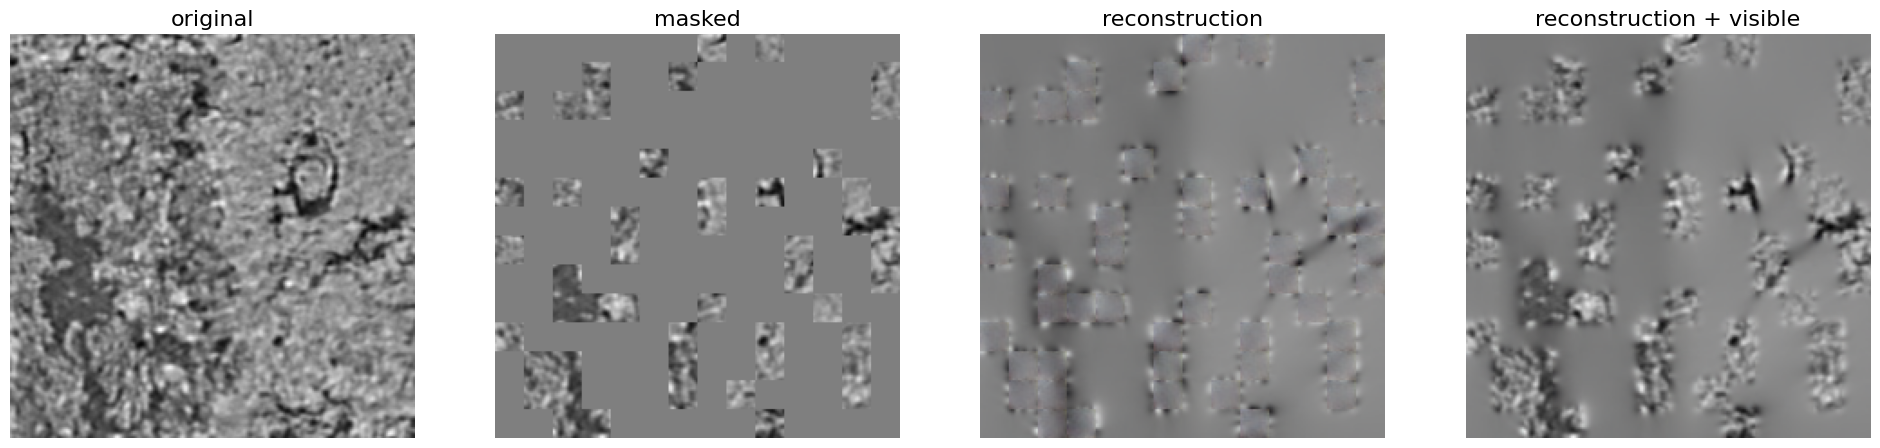
\includegraphics[width=0.9\linewidth]{Figures/Imagenet_example.png}
  \vspace*{1em}
  \caption{Micro-CT reconstruction with model pre-trained on ImageNet.}
  \label{fig:ImageNet}
\end{figure}

The combination of computer vision with medical imaging can benefit the modern medical imaging sector in a variety of ways, including diagnosis, prediction of future outcomes, pathological segmentation from organs to cells, disease monitoring, and so on. Based on the presented challenges of managing micro-CT data, we intend to use computer vision methods, notably autoencoders, to develop an effective approach for compressing and encoding data, as well as to exploit our newly discovered latent representations for further research.


\chapter{Background}
\label{cha:background}

Machine learning is now widely used across many industries, and it has become a powerful tool that may help people in many ways. For example, machine learning techniques can be used to quickly and accurately analyze large amounts of data, while human specialists can continuously evaluate and improve the results. In medical imaging, machine learning has become more and more popular since it can extract important information that helps with precise diagnosis \citep{giger2018machine}. Even though supervised learning has dominated for years, labeling large amounts of training data is becoming prohibitively expensive and time-consuming. As a result, self-supervised learning has become the preferred method for situations involving a moderate amount of annotated data. The following parts introduce the most essential and common self-supervised learning techniques and their applications in medical imaging.

\section{Self-supervised learning}
\label{subsec:self-supervised-learning}

In contrast to supervised learning, self-supervised learning employs labels created from the data itself \citep{ssl_generative_or_contrastive}, negating the need for manual labeling. This possibility leads to more data-efficient models by enabling models to learn from vast amounts of easily accessible data without the requirement for manual annotation. Based on the differences in model structure, self-supervision can be divided into three categories: generative, contrastive, and predictive.

\paragraph{\textbf{Generative Learning}} The generative learning technique arises from the concept that if the model can generate or reconstruct one image, it must have learned something from it. One of the most popular generative models is the autoencoders, which was first introduced by \cite{ballard1987modular} for pre-training artificial neural networks. Autoencoder learns efficient representations by training the network to ignore signal noise. The autoencoder consists of an encoder that compresses the input into a latent representation, and a decoder that reconstructs the input from the latent representation. The goal of the autoencoder is to minimize the reconstruction error, which measures how well the decoder can reproduce the original input. Bidirectional encoder representations from transformers (BERT) \citep{devlin2018bert} is one of the state-of-the-art autoencoder models. Two tasks are used to pre-train BERT \citep{devlin2018bert} on enormous amounts of unlabeled data. The first challenge is masked language modeling, which entails forecasting tokens that have been masked after a certain fraction of input tokens have been hidden. For the model to comprehend sentence relationships, the second challenge is the next sentence prediction. The BERT \citep{devlin2018bert} design is straightforward and effective in trial data. Another popular type of generative model is the auto-regressive model, which predicts the next token in a sequence based on the previous tokens. GPT \citep{brown2020language, radford2018improving, radford2019language} is one of the most prominent examples of auto-regressive models, which also uses a transformer-based neural network to encode and decode the input sequence. Auto-regression models have also been employed in computer vision, such as PixelRNN \citep{van2016pixel} and PixelCNN \citep{van2016conditional}, which use auto-regression methods to model images pixel by pixel. Inspired by the great success of BERT, \cite{he2022masked} proposed a masked autoencoders (MAE) method for computer vision. MAE uses vision transformers as the backbone, masking random patches of the input image and reconstructing the missing pixels to learn the general pattern of the input dataset. 

\paragraph{\textbf{Contrastive Learning}} "Learn to compare" is the goal of contrastive learning \citep{gutmann2010noise}. Using a similarity metric to group similar data closer together and different samples farther apart is the fundamental concept of contrastive learning \citep{jaiswal2020survey}. Given that the data lacks labels, one potential solution to the label problem is the use of pseudo labels, as introduced by Deep Cluster \citep{caron2018deep}. This technique uses clustering to produce pseudo labels, which are then used to ask a discriminator to predict the labels of images. However, this clustering method is time-consuming and performs poorly when compared to later instance discrimination-based algorithms. Instance discrimination methods boost performance by introducing efficient data augmentation strategies. Contrastive multiview coding (CMC) \citep{tian2020contrastive} proposes using multiple views of an image as positive samples and another as negative sample. They discovered that the more views they learned, the better the resultant representation reflected the underlying scene semantics. Similarly, SimCLR \citep{chen2020simple} employs various data augmentation methods, demonstrating the importance of the composition of data augmentation in learning accurate representations. SimCLR \citep{chen2020simple} outperforms CMC \citep{tian2020contrastive} in managing negative samples on a large scale. MoCo \citep{he2020momentum} employs momentum contrast to increase the amount of negative samples. It eliminates the typical end-to-end framework and instead uses two encoders (query and key), which reduces the fluctuation of loss convergence in the initial period.

\paragraph{\textbf{Predictive Learning}} Predicting future or missing information is a frequent strategy for sequential data analysis. Text prediction has been a focus of research in natural language processing for decades. Using a pretext task is the process of creating labels so that supervised approaches can be used in unsupervised situations to train models. According to \cite{mikolov2013efficient}, high-quality word vectors may be trained while reducing computational complexity dramatically. Word2Vec \citep{mikolov2013efficient} uses "center word prediction" as a pretext task. It predicts the missing word between a sequence of words, allowing the model to acquire word representations that may then be used to train models for subsequent tasks. Other language models also use various types of pretext challenges to develop their models' comprehensive sentences. For instance, GPT \citep{brown2020language, radford2018improving, radford2019language} and BERT \citep{devlin2018bert} utilize next word prediction and word prediction from both sides, respectively. 


\section{Vision transformer}
Transformers \citep{vaswani2017attention} are neural network architectures capable of processing sequential data. It was introduced in natural language processing and quickly became the method of choice. However, the application of transformers in computer vision was not very successful until the introduction of Vision Transformers \citep{dosovitskiy2020image}. Transformer's fundamental improvement is the replacement of all recurrent layers with pure attention and fully connected blocks. However, attention does not include a sense of location inside a sequence, therefore, we must add position information to each token. There are many choices of positional encodings, learned and fixed \citep{gehring2017convolutional}. Transformer employs a smart positional encoding method, representing each position with a sinusoid rather than a direct index vector. Sinusoidal position \citep{vaswani2017attention} provides a high value for close tokens that gently decays when one looks at tokens that are further away, and avoids being large in magnitude for extended sequences. The mathematical definition of sinusoidal position is given below:

\begin{gather*}
    P_{(p, 2m)} = \sin \left(\frac{p}{10000 ^ {\frac{2m}{d_{\text{model}}}}}\right) \\
    P_{(p, 2m+1)} = \cos \left(\frac{p}{10000 ^ {\frac{2m}{d_{\text{model}}}}}\right)
\end{gather*}
where \textit{p} is the position, \textit{m} is the dimension, and \(\textit{d}_{\text{model}}\) is the dimension of the output embedding space. Since \(P_{p+k}\) can be expressed as a linear function of \(P_{p}\) for any fixed offset \textit{k}, this enables the model to learn to attend by relative locations.


\section{Self-supervised methods in medical image analysis}
\label{subsec:ssl-medical-imageing}
Medical imaging analysis's main goal is to extract useful data that supports precise diagnosis \citep{anwar2018medical} and facilitates treatment planning and follow-up for clinics. Classification, detection and localization, segmentation, and registration are the four main tasks in medical imaging that sprang out of computer vision tasks \citep{altaf2019going}. However, a significant issue is the lack of high-quality annotated medical imaging datasets. Finding medical images to curate takes a lot of time and money. This is where self-supervised learning comes into play. Self-supervised learning offers the ability to pre-train models so that they capture the general appearance of medical images using the available unlabeled data.

However, self-supervised learning on medical imagery presents various obstacles. Medical images, unlike natural images, appear to be similar. The distinction between healthy and ill patients is based on small visual signals that are highly localized and often difficult to detect \citep{huang2023self}. As a result, some essential phases in self-supervised learning are potentially problematic.

The introduction of several kinds of self-supervised learning used in medical imaging analysis will follow.

\paragraph{\textbf{Generative}} Generative approaches appear to be the least popular method in medical imaging. \cite{chen2019self} developed and validated a novel self-supervised learning technique based on context restoration for classification, localization, and segmentation. They demonstrate that this context restoration strategy outperforms existing pre-training models and provides considerable performance improvements over the baseline. \cite{zhou2023self} proposed self-pre-training using the MAE \citep{he2022masked} approach. They pre-trained a ViT on the target data's training set rather than another dataset, and discovered that MAE self-pre-training significantly improves a variety of medical image tasks such as classification, CT multi-organ segmentation, and MRI brain tumor segmentation.

\paragraph{\textbf{Constrastive}} Contrastive learning is currently the most popular method in medical imaging. Since some standard augmentation methods may be inadequate for medical imaging, instead of building positive pairings with different enhanced versions of the same image, one can improve positive sampling according to the similarity of a patient's clinical information \citep{huang2023self}. For instance, images from the same patient \citep{azizi2021big} and images from patients of similar ages \citep{dufumier2021contrastive}. Some researchers attempted to employ pretext tasks based on natural images as well. Several studies \citep{sowrirajan2021moco, vu2021medaug, chen2021momentum, sriram2021covid} used the MoCo \citep{he2020momentum} framework to create pre-trained models. According to \cite{sowrirajan2021moco}, not all of the augmentation procedures used in the MoCo article are suitable for gray-scale images. \cite{sowrirajan2021moco} solely used random partial rotation and horizontal flipping in their experiments. \cite{sriram2021covid} purely used MoCo \citep{he2020momentum} and trained on non-COVID chest X-ray images. They also used a continuous positional embedding module to extract representations from a collection of time-indexed radiographs. In addition, SimCLR \citep{chen2020simple} is also widely used in medical imaging. \cite{chaitanya2020contrastive} provided two significant improvements by developing domain-specific and problem-specific knowledge simultaneously. The method yields substantial improvements compared
to other self-supervision and semi-supervised learning techniques.

\paragraph{\textbf{Predictive}}Predictive approaches are currently gaining popularity. According to \cite{zhang2017self}, a typical 3D CT or MR volume contains rich context information, which may be easily indexed in 2D slices. The order of slices can be employed in a pretext task to train a predictive self-supervised learning model. This method takes advantage of the particular qualities of medical images and achieves promising results with minimal use
of human annotations. \cite{nguyen2020self} proposed a spatial awareness method that can learn semantic and spatial representations from volumetric medical images. The method consists of two steps: spatial awareness learning and semantic feature learning. In the first step, the method randomly crops four patches from an input image and predicts their relative positions using a convolutional neural network (CNN). This task forces the network to learn the spatial structure and layout of the image. In the second step, the method uses the same CNN to extract semantic features from the whole image and compares them with the features of another image using a contrastive loss function. This task encourages the network to learn discriminative and robust features that can distinguish different images. The results showed that the proposed method can improve the performance of organ segmentation and intracranial hemorrhage detection tasks by using the learned features as initialization or regularization for the supervised models.


\chapter{Methodology}

The micro-CT data used in this project offers exceptional resolution and includes information from both low and high magnification. For a medical task, both types of information may be relevant for certain activities, so we want to keep multiscale data. However, because this data is not manageable in size, we wish to first divide the entire image into manageable-sized chunks. We opted to try out the masked autoencoder (MAE)\citep{he2022masked} technique in the project.

The decision to attend MAE was motivated by two factors. First, patch-based processing allows the model to collect implicit information at low magnification. Masking certain parts encourages the model to learn the full-scale information as well. This coincides with our goal of preserving multiscale data. Second, the structure of MAE is quite straightforward and easy to develop. Furthermore, the structure of the model considerably reduces the computational resources it requires. 

\section{Masked autoencoder}

Masked autoencoder is a simple autoencoding approach that reconstructs the original input signal given its partial observation. MAE consists of an encoder and a decoder. The encoder part of the MAE transforms the visible image patches into a latent representation of \textit{M} dimensions. This representation is later used as input for the decoder so that the decoder can reconstruct the whole input image. The structure of MAE is illustrated in Figure \ref{fig:MAE}.

\begin{figure}[t]
  \centering
  \vspace*{1em}
  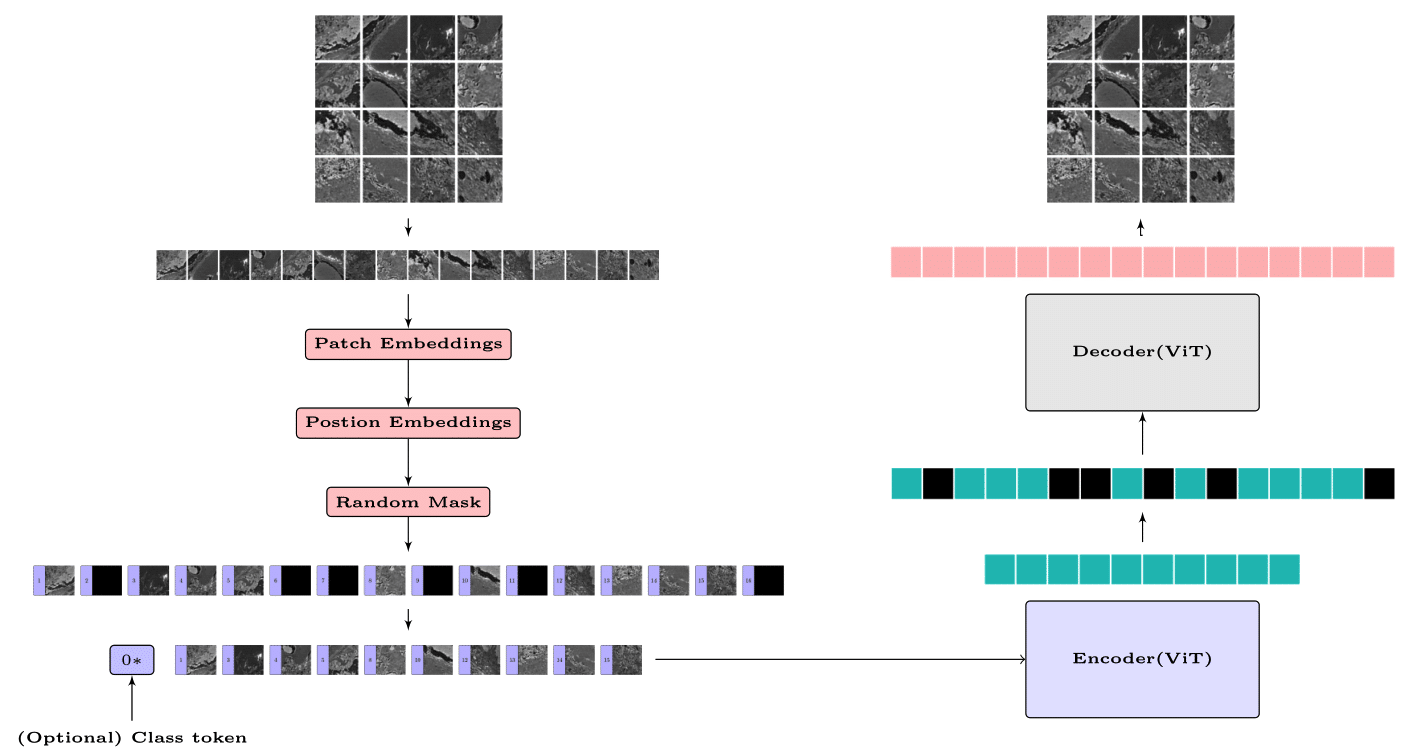
\includegraphics[width=1.0\linewidth]{Figures/model_structure.png}
  \vspace*{1em}
  \caption{MAE architecture illustration.}
  \label{fig:MAE}
\end{figure}

MAE relies on vision transformers (ViT) \citep{dosovitskiy2020image} as its foundation. First, we partition the image into non-overlapping patches. As in a standard ViT, we project these patches into vectors and add a fixed sinusoidal position \citep{vaswani2017attention} to each one. In this method, we provide our model with relative location information, allowing it to retain knowledge of patch order. Figure \ref{fig:pos_embed} shows an example of embedded position information. Then we sample a subset of patches and mask (i.e., remove) the remainder. The masking strategy is simple: generate random numbers between $(0, 1)$ using a uniform distribution, take these numbers as the index of tokens, sort them in ascending order, and then remove a specified percentage of the input tokens.

\begin{figure}[t]
  \begin{center}
    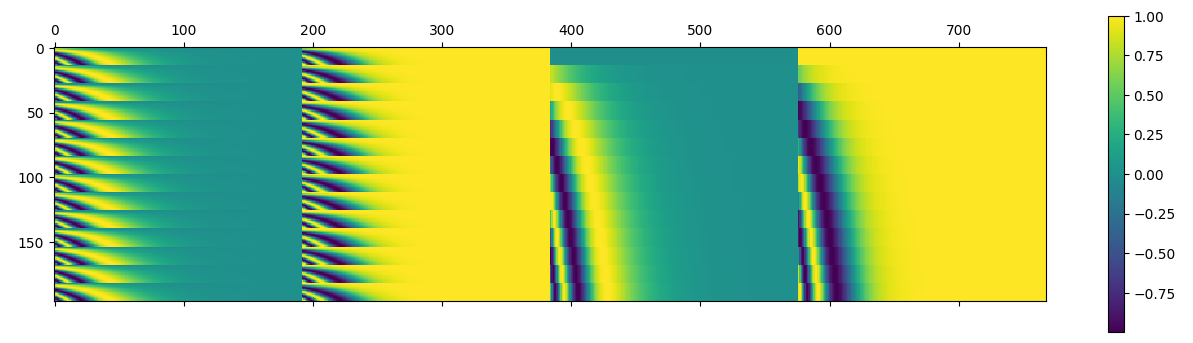
\includegraphics[width=1.0\textwidth]{Figures/pos_embed.png}
  \end{center}
  \caption{Position embedding visualization for input data.}
  \label{fig:pos_embed}
\end{figure}

By randomly masking a high percentage of patches (in our example $70\%$), our encoder acts on a small part of the overall set, significantly lowering the processing resources required. This allows us to train enormously large encoders with a fraction of the computational resources and memory. Random masking also plays an important function in eliminating redundancy. Unlike texts, images have low semantic information, thus we must manually design a difficult assignment to encourage the model to learn high-level semantic information, instead of simply reconstructing the missing pixels from neighboring patches.

The encoder is simply a standard ViT \citep{dosovitskiy2020image} applied exclusively to visible patches. Following the ViT \citep{dosovitskiy2020image} steps, the encoder embeds patches using a linear projection with extra positional embeddings, and then processes the resulting set using a sequence of Transformer blocks. As previously stated, our encoder only operates on a small subset of the total input patches, all masked tokens are eliminated, and no mask tokens are used. A lightweight decoder handles the entire set.

Figure \ref{fig:MAE} illustrates how the decoder handles all tokens. Each masked token is a common, learnt vector that signals the presence of a missing patch that must be predicted. By adding position embeddings to all tokens in this whole set, masked tokens may determine where they belong in the image. This masked set, along with the encoded visible tokens, passes through the decoder Transformer blocks to produce the reconstructed input image. Moreover, the decoder is independent of the encoder, so the architecture can be flexibly designed. In the experiment, we used a shallower and narrower decoder to process the whole set, which reduces the pre-training time.

The MAE decoder reconstructs the input by predicting the pixel values of each masked patch. The decoder's output contains a vector of pixel values representing a patch. The decoder output is reshaped to provide a reconstructed image. We employ mean squared error: 
\begin{equation}
        \mathcal{L} = \frac{1}{n} \sum_{i=1}^{n} (y_i - \hat{y}_i)^2
\end{equation}
to compute the loss between the reconstructed and original images in pixel space. We calculate the loss just on masked patches.

\textbf{TODO}
\begin{itemize}
    \item Augmentation of the input images
    \item Clustering method
\end{itemize}


\chapter{Experiments}
\section{Set up}
\label{experiments set up}

We do self-supervised pre-training on the micro-CT dataset. Then we perform clustering on the same dataset but with unseen data (different parts of the slices). 

\section{Model training}
\label{model training}

\begin{figure}[t]
  \begin{center}
    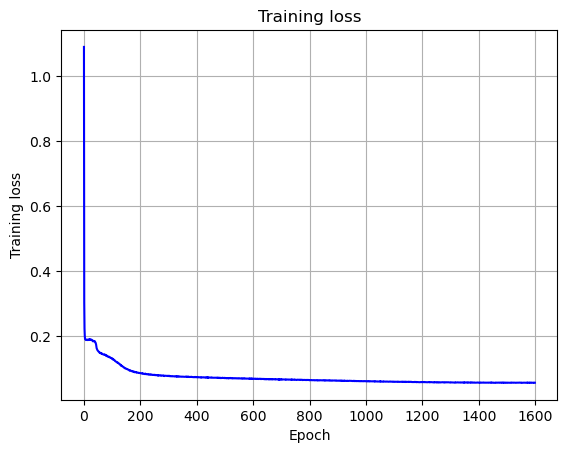
\includegraphics[width=0.9\textwidth]{Figures/loss.png}
  \end{center}
  \caption{Training loss per epoch.}
  \label{fig:training loss}
\end{figure}

\section{Main Properties}
\label{main properties}

\begin{figure}[H]
  \centering
  \begin{tabular}{@{\hspace{2pt}}c@{\hspace{3pt}}c@{\hspace{2pt}}c@{\hspace{2pt}}c@{\hspace{2pt}}c@{\hspace{2pt}}c@{\hspace{2pt}}c@{\hspace{2pt}}c}
    \rule{0pt}{0pt} \makecell{Patch size \\ $(16 \times 16)$} & 
        \adjincludegraphics[width=.25\linewidth,valign=c]{Figures/patch16_mask.png} &
        \adjincludegraphics[width=.25\linewidth,valign=c]{Figures/patch16_rec.png} &
        \adjincludegraphics[width=.25\linewidth,valign=c]{Figures/original_input.png} \\

    \rule{0pt}{30pt} \makecell{Patch size \\ $(8 \times 8)$}& 
        \adjincludegraphics[width=.25\linewidth,valign=c]{Figures/patch_8_mask.png} &
        \adjincludegraphics[width=.25\linewidth,valign=c]{Figures/patch_8_rec.png} &
        \adjincludegraphics[width=.25\linewidth,valign=c]{Figures/original_input.png} \\

    \rule{0pt}{20pt} & \textbf{mask} & \textbf{reconstruction} & \textbf{groudtruth} \\
  \end{tabular}
  \caption{Results of reconstructed images with different patch size.}
    \label{fig:results with different patch size}
\end{figure}


\chapter{Implementation}


\chapter{Discussion}


\chapter{Conclusion}


\bibliographystyle{agsm}
\bibliography{references}
\end{document}

%%% Local Variables: ***
%%% mode: latex ***
%%% TeX-master: "main.tex"  ***
%%% ispell-local-dictionary: "british"  ***
%%% End: ***